%----------------------------------------------------------------------------------------
% METADATA BLOCK (YAML)  — see inbox/README.md for every field
%----------------------------------------------------------------------------------------
% uid: ""
% school: "lycee"
% level: "4eme"
% section: "Mathématiques"
% chapter: "Nombres complexes"
% title: "Le couple de Tusi"
% difficulty: "Moyen"
% tags: ["tusi", "hypocycloide", "ellipse", "astroide", "nombres-complexes"]
% provenance: "adapted"
% batch: "2026-11-20-defis-geometrie-A"
% defi: true
%----------------------------------------------------------------------------------------

\newcommand{\C}{\mathbb{C}}

% ---STATEMENT---
Le plan est identifié à $\C$ ; $O$ est l'origine. Un cercle $\gamma$ de rayon $r$ roule sans glisser, à l'intérieur d'un cercle fixe $\Gamma$ de centre $O$ et de rayon $R=nr$ ($n\in\{2,3,4\}$). Initialement, $\gamma$ est tangent à $\Gamma$ au point $(R,0)$ et un point $M$ de $\gamma$ est confondu avec ce point de contact. On note $C$ le centre de $\gamma$ et $t$ l'angle $\left(\vec{\imath},\overrightarrow{OC}\right)$, avec $t\geq0$.

% alt: Cercle fixe de rayon 2r et cercle mobile de rayon r roulant à l'intérieur, point M du cercle mobile sur le diamètre horizontal
\begin{center}
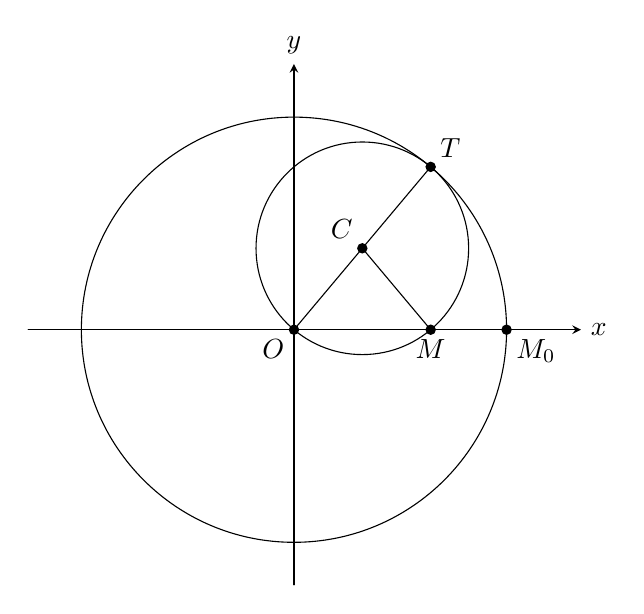
\begin{tikzpicture}[scale=1.35,line cap=round,line join=round,>=stealth]
\draw (0,0) circle (2);
\draw (0.643,0.766) circle (1);
\draw[->] (-2.5,0) -- (2.7,0) node[right]{$x$};\draw[->] (0,-2.4) -- (0,2.5) node[above]{$y$};
\draw[thin] (0,0) -- (1.286,1.532);
\draw[thin] (0.643,0.766) -- (1.286,0);
\fill(0,0) circle (1.4pt) node[below left] {$O$};
\fill(0.643,0.766) circle (1.4pt) node[above left] {$C$};
\fill(1.286,1.532) circle (1.4pt) node[above right] {$T$};
\fill(1.286,0) circle (1.4pt) node[below] {$M$};
\fill(2,0) circle (1.4pt) node[below right] {$M_0$};
\end{tikzpicture}
\end{center}

\begin{enumerate}
  \item Exprimer l'affixe de $C$ en fonction de $t$. En écrivant que $\gamma$ roule sans glisser (les arcs parcourus sur $\Gamma$ et sur $\gamma$ ont même longueur), montrer que l'affixe de $M$ est
  \[z(t)=(R-r)\,e^{it}+r\,e^{-i\,\frac{R-r}{r}\,t}.\]
  \item \textbf{Cas $n=2$.} Montrer que $M$ glisse sur un diamètre de $\Gamma$.
  \item \textbf{Autres points.} Soit $Q$ un point lié à $\gamma$, à la distance $\rho\neq r$ de $C$ (initialement $\overrightarrow{CQ}$ fait un angle $\varphi$ avec $\overrightarrow{CM}$, dans le sens direct). Montrer que, pour $n=2$, $Q$ décrit une ellipse dont on précisera les demi-axes.
  \item \textbf{Cas $n=3$ et $n=4$.} Écrire $z(t)$. Montrer que pour $n=4$ la courbe a pour équation cartésienne $x^{2/3}+y^{2/3}=(4r)^{2/3}$ (astroïde), et que pour $n=3$ elle admet exactement trois points de rebroussement (deltoïde).
\end{enumerate}

% ---SOLUTION---
\begin{enumerate}[itemsep=14pt]
  \item $C$ est à la distance $R-r$ de $O$ (cercles tangents intérieurement) et l'angle $\left(\vec\imath,\overrightarrow{OC}\right)$ vaut $t$ : l'affixe de $C$ est $(R-r)e^{it}$.

  Le point de contact est $T=Re^{it}$. L'arc de $\Gamma$ parcouru depuis $(R,0)$ jusqu'à $T$ mesure $Rt$.

  \begin{prop}[Roulement sans glissement]
  Les arcs parcourus ont la même longueur. Un arc de cercle de rayon $\rho$ et d'angle $\psi$ mesure \ib{$\rho\,\psi$}.
  \end{prop}
  Sur $\gamma$, l'arc entre $M$ et le point de contact $T$ mesure aussi $Rt$ : il a pour angle $\psi=\dfrac{Rt}{r}$. Vu de $C$, le point de contact est dans la direction $e^{it}$ et $M$ est en retard de cet angle (parcouru dans le sens direct de $M$ vers $T$) :
  \[\overrightarrow{CM}=r\,e^{i\left(t-\frac{R}{r}t\right)}.\]
  Or $t-\dfrac Rr\,t=-\dfrac{R-r}{r}\,t$. Donc, comme $z(t)=\text{affixe de }C+\text{affixe de }\overrightarrow{CM}$,
  \[\ib{$z(t)=(R-r)e^{it}+r\,e^{-i\frac{R-r}{r}t}$}.\]

  \item $R=2r$ : $\dfrac{R-r}{r}=1$ et $z(t)=r e^{it}+r e^{-it}=2r\cos t$.

  Cet affixe est réel : $M$ reste sur l'axe des abscisses, et $2r\cos t$ parcourt $[-2r,2r]$ : \ib{$M$ glisse sur un diamètre de $\Gamma$}.

  \item L'affixe de $Q$ est $z_Q=(R-r)e^{it}+\rho\,e^{i\left(\varphi-\frac{R}{r}t+t\right)}$ ; pour $n=2$ ($R=2r$) : $z_Q=r e^{it}+\rho\,e^{i(\varphi-t)}$.

  On tourne le repère de l'angle $\dfrac\varphi2$ : $Z=z_Qe^{-i\varphi/2}$. Posons $\tau=t-\dfrac\varphi2$ :
  \[Z=r e^{i\tau}+\rho\,e^{-i\tau}=(r+\rho)\cos\tau+i\,(r-\rho)\sin\tau.\]
  \begin{prop}[Ellipse]
  Les points $(X,Y)=(a\cos\tau,\ b\sin\tau)$, $a,b>0$, décrivent l'ellipse d'équation \ib{$\dfrac{X^2}{a^2}+\dfrac{Y^2}{b^2}=1$}.
  \end{prop}
  Donc $Q$ décrit, dans le repère tourné de $\dfrac\varphi2$, l'ellipse $\dfrac{X^2}{(r+\rho)^2}+\dfrac{Y^2}{(r-\rho)^2}=1$, de centre $O$ et de demi-axes \ib{$r+\rho$ et $|r-\rho|$}.

  Si $\rho=r$, le demi-petit axe est nul : c'est le segment de la question 2. Si $\rho=0$ ($Q=C$), c'est le cercle de rayon $r$.

  \item Pour $R=nr$ : $z(t)=(n-1)r\,e^{it}+r\,e^{-i(n-1)t}$.

  \emph{$n=4$ :} $z(t)=3r\,e^{it}+r\,e^{-3it}$ donc
  \[x=r(3\cos t+\cos3t)=4r\cos^3t,\qquad y=r(3\sin t-\sin3t)=4r\sin^3t,\]
  car $\cos3t=4\cos^3t-3\cos t$ et $\sin3t=3\sin t-4\sin^3t$. Alors $x^{2/3}+y^{2/3}=(4r)^{2/3}(\cos^2t+\sin^2t)=(4r)^{2/3}$ : \ib{$astroïde$}.

  \emph{$n=3$ :} $z(t)=2r\,e^{it}+r\,e^{-2it}$ et $z'(t)=2ir\,e^{it}-2ir\,e^{-2it}=2ir\,e^{-it/2}\left(e^{3it/2}-e^{-3it/2}\right)=-4r\,e^{-it/2}\sin\dfrac{3t}2$.

  $z'(t)=0\iff\sin\dfrac{3t}{2}=0\iff t=\dfrac{2k\pi}{3}$, ce qui donne trois valeurs de $z$ (pour $k=0,1,2$) : \ib{$trois points de rebroussement$}, la courbe est un deltoïde. $\blacksquare$
\end{enumerate}

\textbf{Remarque.} Le deltoïde obtenu pour $n=3$ est la courbe enveloppe des droites de Simson d'un triangle (résultat classique, admis) ; l'astroïde ($n=4$) a quatre rebroussements ($z'(t)=0\iff\sin2t=0$).

\textbf{Idée :} le roulement sans glissement impose que la rotation propre de $\gamma$ est $-\dfrac{R-r}{r}t$ ; pour $R=2r$ elle vaut exactement $-t$, ce qui replie l'orbite sur un segment.

\textbf{Piège :} le sens de rotation de $\gamma$ est \emph{opposé} à celui de $C$ autour de $O$ ; d'où le signe $-$ dans l'exponentielle.
